\chapter{Preliminaries}
\label{cha:preliminaries}
This chapter lays the theoretical foundations required to understand the proposed methodology.
It bridges the geophysics of planetary Radar Sounders (RS)---which govern signal formation and subsurface probing---with the mathematical framework of deep generative models used for image-to-image translation.
Section~\ref{sec:planetary_radar_sounders} first describes the physics of radargram acquisition, from electromagnetic propagation to clutter formation.
Section~\ref{sec:rs_challenges} then highlights RS-specific challenges that motivate specialized deep learning approaches.
Finally, Section~\ref{sec:dl_theory} introduces the key DL concepts---CNNs, U-Net architectures, and GANs---that underpin the Sim-to-Real pipeline developed in Chapter~\ref{cha:methodology}.

\section{Planetary Radar Sounders}
\label{sec:planetary_radar_sounders}
Planetary Radar Sounders (RS) are nadir-looking, low-frequency radar instruments specifically designed to probe the shallow subsurface of planetary bodies from orbit.
By transmitting short radio pulses in the HF–VHF bands (typically in the range 1–30~MHz) and recording the time-delayed echoes, RS instruments acquire  radargrams that represent the dielectric structure along the spacecraft ground track.
In contrast to Synthetic Aperture Radar (SAR) systems, which operate at higher frequencies and synthesize an along-track aperture to image surface backscatter, Radar Sounders trade azimuth resolution for increased penetration depth .

Representative examples of orbital Radar Sounders include MARSIS\cite{Jordan_2009} (Mars Advanced Radar for Subsurface and Ionosphere Sounding) on board \emph{Mars Express}\cite{ESA_MarsExpress} and SHARAD (SHAllow RADar)\cite{Seu_2007} on board \emph{Mars Reconnaissance Orbiter}\cite{Zurek_2007}.
Both instruments have demonstrated the capability to detect subsurface layering, buried basins, and potential volatile reservoirs on Mars, and similar sounders have been proposed or deployed for other planetary bodies.
In this work, we specifically focus on SHARAD, whose data are described in detail in Section~\ref{sec:dataset}, but the physical principles outlined below apply more generally to planetary RS systems.

\subsection{Electromagnetic Wave Propagation}
\label{subsec:em_propagation}
Radar Sounders operate by exploiting the interaction between electromagnetic waves and dielectric materials, which governs both wave propagation and echo formation.
The propagation of a radar signal through a medium is governed by its complex dielectric permittivity $\epsilon^*$, defined as:
\begin{equation}
\epsilon^* = \epsilon' - j\epsilon''
\end{equation}
where $\epsilon'$ is the real part (dielectric constant), which controls the phase velocity of the wave and thus the apparent depth of reflectors, and $\epsilon''$ is the imaginary part (dielectric loss factor), which controls the attenuation of the signal amplitude, and therefore the reflected power that can be measured at a given depth.

The velocity $v$ of the electromagnetic wave in a medium is given by:
\begin{equation}
v = \frac{c}{\sqrt{\epsilon'}}
\end{equation}
where $c \approx 3 \times 10^8$~m/s is the speed of light in vacuum.
This relationship is crucial for converting the temporal delay of radar echoes into geometric depth: a given sampling interval in time $\Delta t$ corresponds to a range sampling interval
\begin{equation}
\Delta r = \frac{v}{2}\,\Delta t = \frac{c}{2\sqrt{\epsilon'}}\,\Delta t,
\end{equation}
where the factor $1/2$ accounts for the two-way travel path (down and up).

Typical values of $\epsilon'$ and the corresponding phase velocities are reported below:
\begin{itemize}
    \item \textbf{Air / Vacuum:} $\epsilon' \approx 1$, $v \approx c \approx 3.0 \times 10^8$~m/s.
    \item \textbf{Liquid water:} $\epsilon' \approx 80$ at radio frequencies, $v \approx 3.3 \times 10^7$~m/s.
    \item \textbf{Pure water ice:} $\epsilon' \approx 3.1$–$3.2$, $v \approx 1.7 \times 10^8$~m/s.
    \item \textbf{Basaltic rock / dry regolith:} $\epsilon' \approx 4$–$8$ (depending on porosity and composition), $v \approx (1.1$–$1.5) \times 10^8$~m/s.
\end{itemize}

\begin{table}[t]
    \centering
    \caption{Typical values of relative dielectric permittivity $\epsilon'$ and corresponding phase velocity $v$ for materials relevant to planetary Radar Sounder applications.}
    \label{tab:dielectric_constants}
    \begin{tabular}{lcc}
        \hline
        Material                & $\epsilon'$ (–) & $v$ [m/s] \\
        \hline
        Vacuum / Air            & $\approx 1.0$   & $\approx 3.0 \times 10^8$ \\
        Liquid water            & $\approx 80$    & $\approx 3.3 \times 10^7$ \\
        Pure water ice          & $\approx 3.1$–$3.2$ & $\approx 1.7 \times 10^8$ \\
        Dry basaltic rock       & $\approx 6$–$8$ & $\approx (1.1$–$1.2) \times 10^8$ \\
        Porous dry regolith     & $\approx 3$–$5$ & $\approx (1.3$–$1.7) \times 10^8$ \\
        Ice–dust mixtures (Mars)& $\approx 3$–$6$ & $\approx (1.2$–$1.7) \times 10^8$ \\
        \hline
    \end{tabular}
\end{table}

On Mars, the shallow subsurface is expected to consist of mixtures of basaltic material, dust, and water ice, leading to effective dielectric constants in the range $\epsilon' \approx 3$–$6$ for many geologic units.
As a consequence, the apparent depth corresponding to a given time delay can vary significantly between terrains dominated by ice (higher velocity, larger depth per sample) and those dominated by rock or dust (lower velocity, smaller depth per sample).

\subsection{Reflection and Transmission}
When the propagating wave encounters an interface between two layers with different dielectric constants ($\epsilon'_1$ and $\epsilon'_2$), a portion of the electromagnetic energy is reflected back towards the Radar Sounder and a portion is transmitted into the second medium.
The first interface encountered is invariably between vacuum/air ($\epsilon'_1 \approx 1$) and the planetary surface material ($\epsilon'_2 \gg 1$), producing a strong reflection due to the large dielectric contrast.
Subsequent subsurface interfaces typically exhibit weaker contrasts.
For normal incidence, the amplitude of the reflected field is determined by the Fresnel reflection coefficient $R$:
\begin{equation}
R = \frac{\sqrt{\epsilon'_1} - \sqrt{\epsilon'_2}}{\sqrt{\epsilon'_1} + \sqrt{\epsilon'_2}}.
\end{equation}
A strong reflection (large $|R|$) implies a significant contrast in dielectric properties (e.g., ice/basalt interface), while weak reflections suggest gradual transitions or similar materials.

The fraction of power that is not reflected at the interface is transmitted into the second medium.
However, during propagation in this medium, the transmitted energy can be progressively reduced by several mechanisms, including material absorption (related to $\epsilon''$), volume scattering from inhomogeneities, and small-scale roughness that redirects energy away from the nadir direction.
These effects are collectively described by an attenuation factor, which causes the amplitude (and thus the reflected power) of echoes from deeper interfaces to decrease approximately exponentially with depth.

For RS applications, the observable echoes from both surface and subsurface interfaces result from the combination of:
\begin{itemize}
    \item the radar equation, which accounts for transmitted power, antenna gains, and range-dependent geometric spreading of the wavefront,
    \item the reflection coefficient at the interface (dielectric contrast),
    \item the cumulative attenuation along the propagation path.
\end{itemize}
Interfaces with modest dielectric contrast can still produce detectable echoes if the overlying medium is weakly attenuating (e.g., cold, pure ice), whereas even strong contrasts may become undetectable if the path includes highly lossy materials.

\subsection{Radargrams}
A \textbf{radargram} is the two-dimensional representation of the echoes acquired by an RS along the spacecraft ground track.
Each column of the radargram corresponds to a single range profile, called\emph{Rangeline} or \emph{A-scan}, while each row corresponds to a fixed time delay (and thus an approximate depth) sampled at regular intervals.

From a signal-processing viewpoint, a radargram is therefore organized along two principal dimensions: the \emph{fast-time} (range) axis, associated with echo delay and depth, and the \emph{slow-time} (along-track) axis, associated with the motion of the platform.
In more detail:
\begin{itemize}
    \item \textbf{Rangeline / A-scan (fast time):} For each transmitted pulse, the RS records the received voltage (or power) as a function of time delay $\tau$, sampled at a fixed sampling frequency $f_s$. This one-dimensional array of samples forms a single rangeline, describing the echo strength as a function of range. The sampling interval in time is $\Delta t = 1/f_s$, which corresponds, as already introduced in Section~\ref{subsec:em_propagation}, to a range sampling interval
    \begin{equation}
        \Delta r = \frac{c}{2\sqrt{\epsilon'}}\,\Delta t,
    \end{equation}
    where $\epsilon'$ is an effective dielectric constant for the medium.
Different materials correspond to different propagation velocities and thus to different depth-per-sample relationships.
    \item \textbf{Slow time (along-track):} As the spacecraft moves along its orbit, successive pulses are transmitted at a Pulse Repetition Frequency (PRF) and the corresponding rangelines are acquired at different along-track positions.
Stacking these rangelines side by side yields the 2D radargram, whose horizontal axis represents slow time (or along-track distance) and whose vertical axis represents fast time (or range).
\end{itemize}

Beyond individual 2D radargrams, suitably processed collections of RS acquisitions can be combined into three-dimensional \emph{C-scan} volumes, in which multiple radargrams are stacked in the cross-track direction to form a tensor representation of the subsurface~\cite{yebasse2025advances}.
Such 3D products, for example the volumetric reconstructions of the Martian polar caps derived from SHARAD data provided by the US science team~\cite{foss2017sharad3d}, enable true volumetric analysis of layering and buried structures while retaining the radargram as their fundamental building block.

The intensity of each pixel in a radargram corresponds to the power of the received echo at a given time delay and along-track position, typically expressed in logarithmic scale (dB) to compress the wide dynamic range of the signal. Bright, nearly horizontal features often correspond to strong, laterally continuous reflectors such as the surface or major subsurface interfaces, while hyperbolic patterns are typically produced by point-like or small-scale scatterers.
Understanding how acquisition parameters (sampling rate, PRF, spacecraft velocity) map into the sampling grid of the radargram is essential for correctly interpreting reflector geometry and for designing processing algorithms that operate in the radargram domain.

\subsection{Resolution and Clutter}
The ability to resolve features in range is defined by the system's bandwidth $B$.
In pulse-compression radar sounders, this bandwidth is typically achieved by transmitting a linear frequency-modulated (chirp) signal and applying matched filtering at reception, so that the attainable range resolution is
\begin{equation}
    \Delta r = \frac{c}{2B\sqrt{\epsilon'}}
\end{equation}
For SHARAD ($B = 10$~MHz), the vertical resolution in free space is approximately 15~m.
In ice ($\epsilon' \approx 3.15$), this improves to $\approx 8.4$~m \cite{Seu_2007}.
The along-track (azimuth) resolution is determined by the effective antenna footprint and the details of the coherent processing.

A critical challenge in RS is \textbf{surface clutter}.
Reflections from off-nadir topographic features (e.g., mountains, crater rims, rough volcanic terrains) can reach the receiver with the same time delay as nadir subsurface echoes.
These \enquote{ghost} signals can be misinterpreted as deep aquifers or layers.
Importantly, the RS footprint on the surface is not point-like: each transmitted pulse illuminates an extended area around the nadir track, whose size depends on antenna beamwidth, altitude, and frequency.
Within this footprint, echoes originate from a continuum of incidence angles, including contributions from slopes and rough facets that are significantly displaced from the nadir point.

As the spacecraft moves along its orbit and pulses are transmitted at the Pulse Repetition Frequency (PRF), successive, partially overlapping footprints are sampled and coherently combined.
This synthetic focusing improves along-track resolution but does not entirely eliminate contributions from off-nadir scatterers, especially over rough or highly structured terrain.
The combined effect is that a single pixel in the radargram may integrate energy from multiple scattering centres at different lateral positions, complicating the direct inversion from image space to subsurface structure.

\begin{figure}[ht]
    \centering
    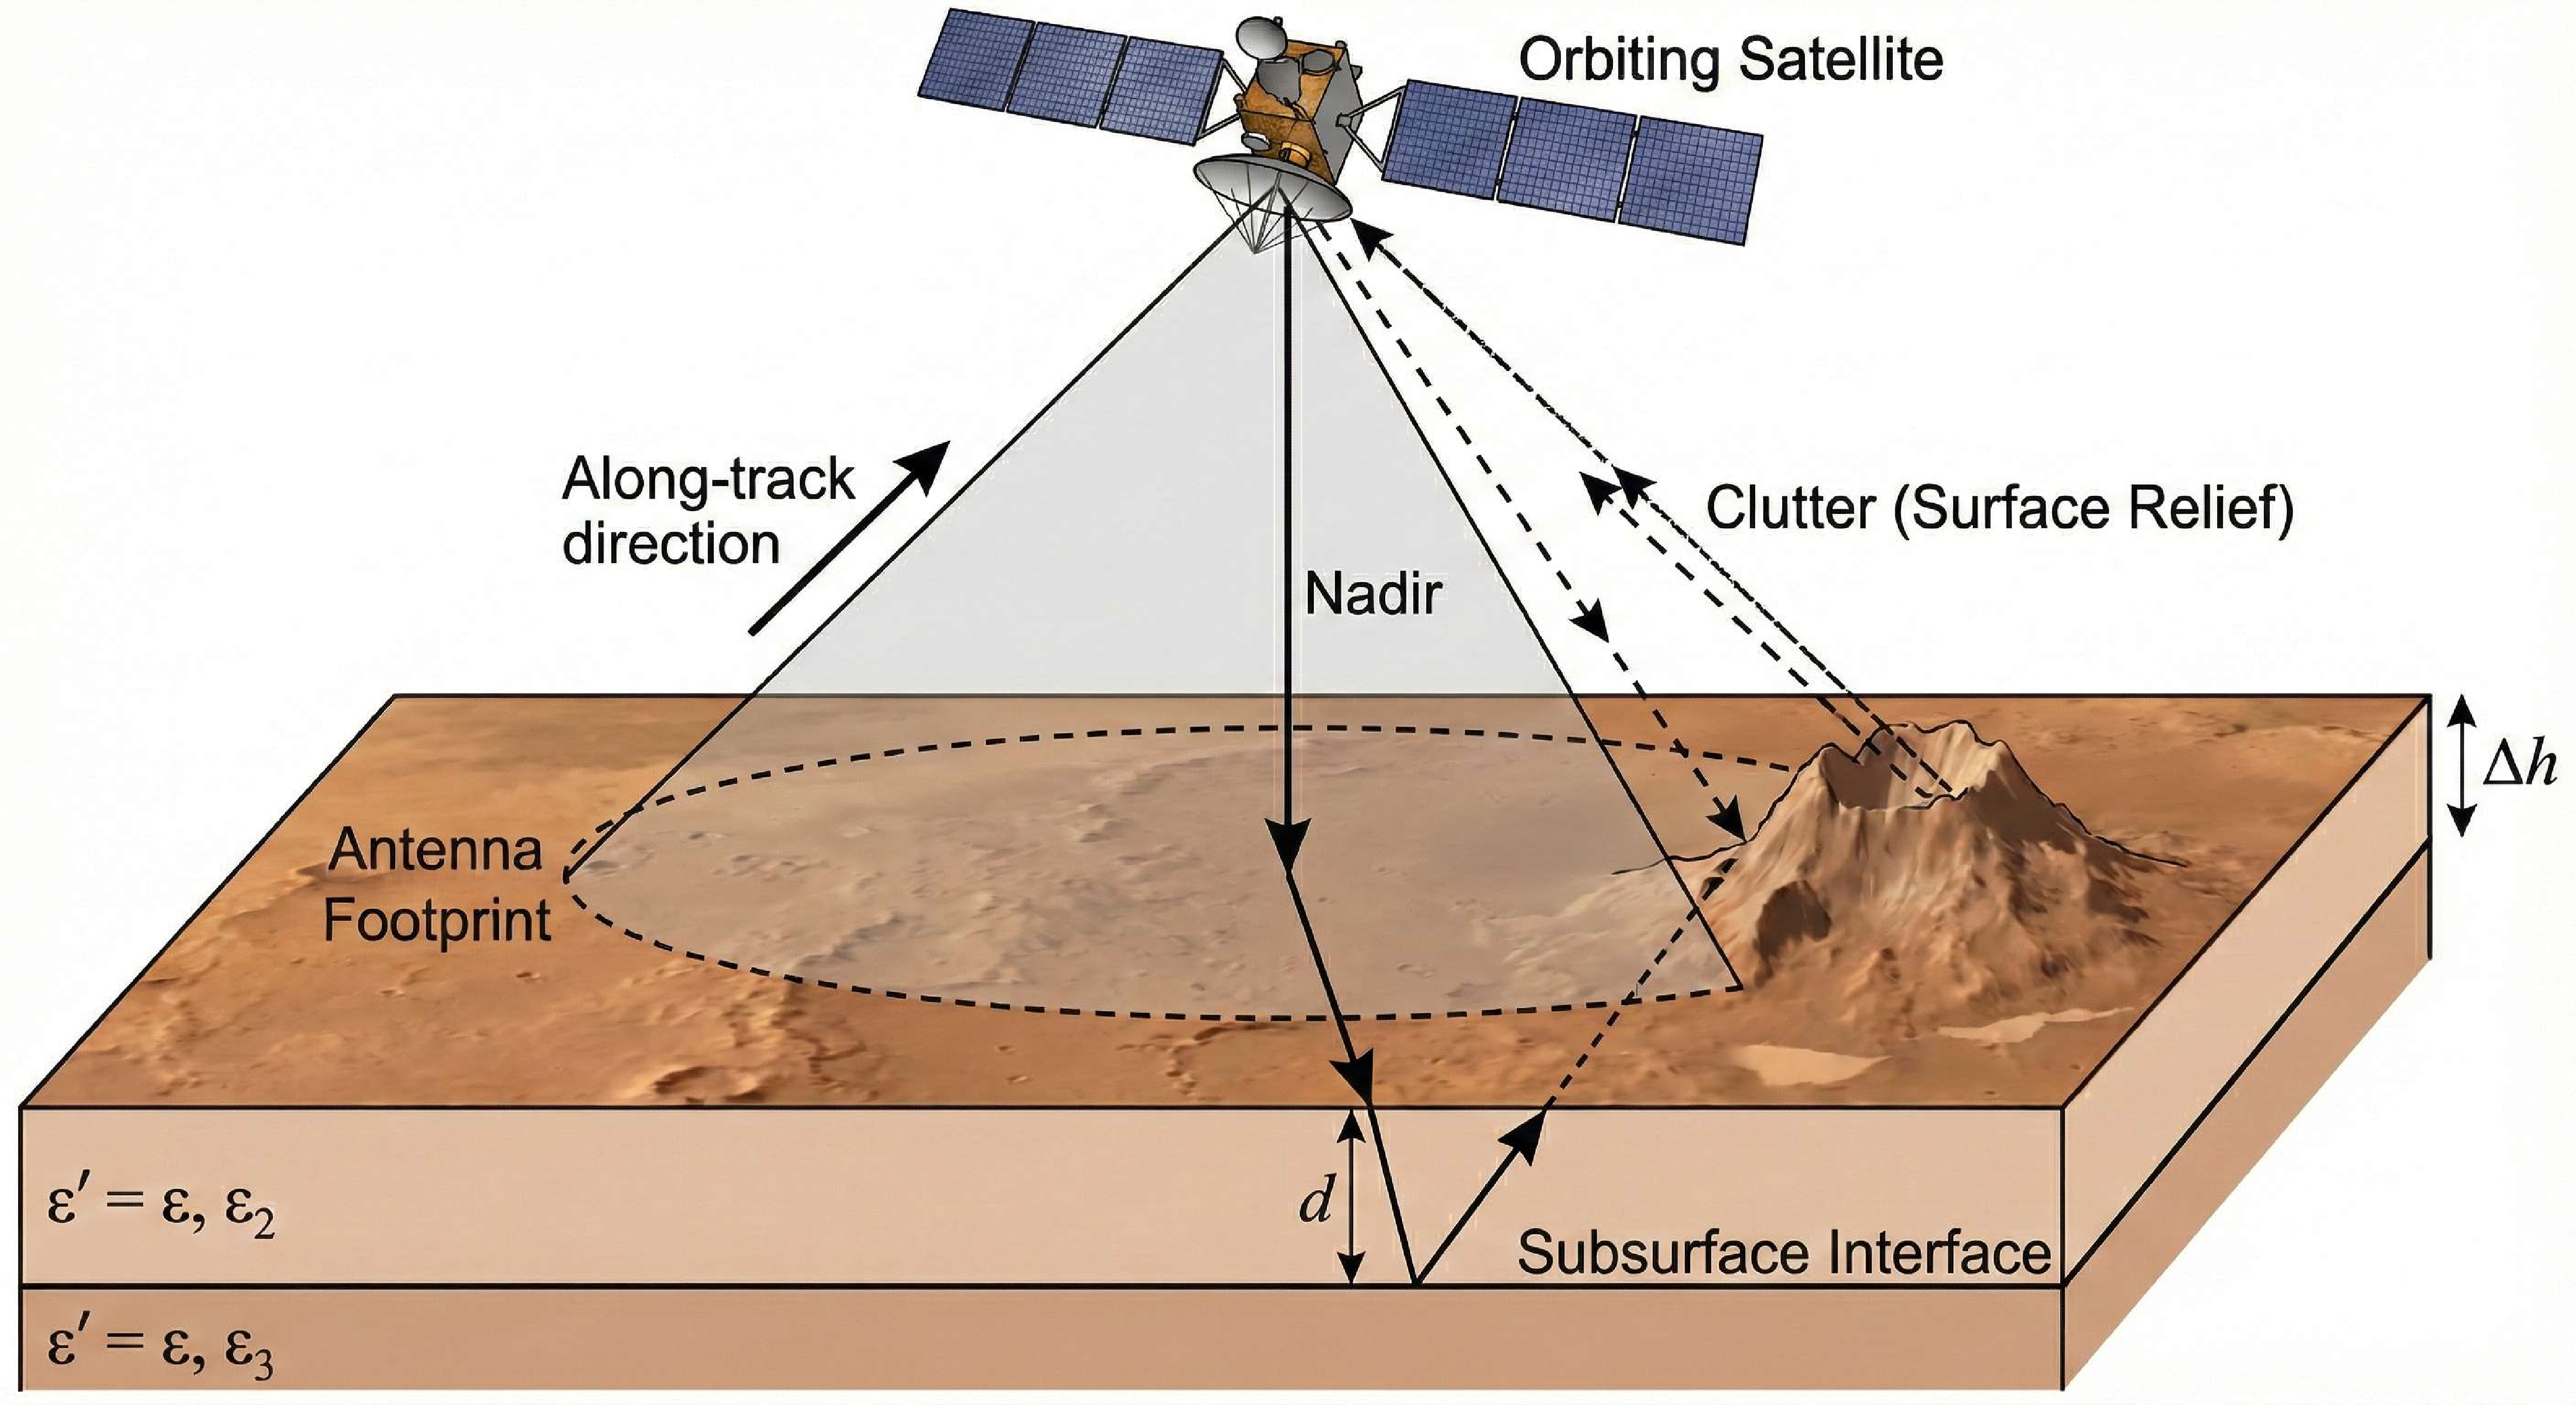
\includegraphics[width=1\linewidth]{images/Gemini_Generated_Image.pdf}
    \caption{Conceptual illustration of a planetary Radar Sounder (RS) acquisition geometry. The nadir-looking instrument transmits pulses that interact with dielectric interfaces in the subsurface (e.g., at depth $d$), returning time-delayed echoes to the receiver \cite{Seu_2007, Daniels_2004}. Due to the finite effective antenna footprint, off-nadir surface topographic features (such as relief with height $\Delta h$) can generate reflections \cite{Seu_2007, foss2017sharad3d}. These ``surface clutter'' signals can arrive at the same time delay as genuine nadir subsurface echoes, complicating data interpretation \cite{foss2017sharad3d, yebasse2025advances}.}
    \label{fig:rs_geometry_clutter}
\end{figure}


\section{Specific Challenges of RS Data}
\label{sec:rs_challenges}
The application of computer vision techniques, originally developed for natural optical imagery, to RS data presents a number of domain-specific challenges. 

\begin{figure}[t]
    \centering
    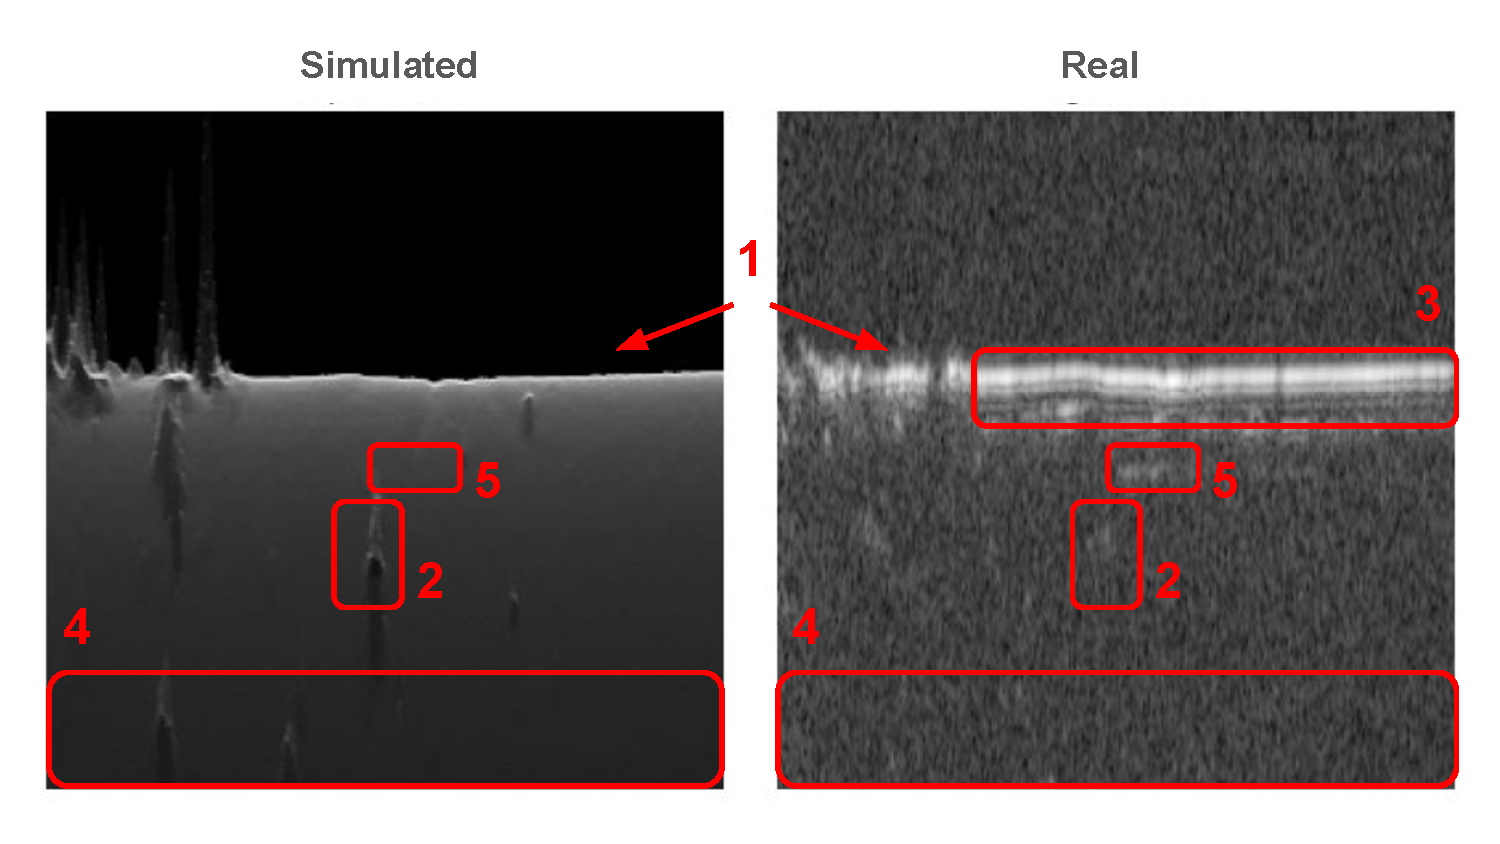
\includegraphics[width=\linewidth]{images/sim_real_radargram_annotated}
    \caption{Example of a simulated (left) and real (right) radargram patch from the Elysium Planitia study region, with key features and challenges highlighted. 
    (1) The bright surface return is clearly visible in both cases, though it appears more diffuse in the real data due to speckle noise and surface roughness. 
    (2) An isolated clutter point, correctly predicted and sharply rendered in the simulated radargram, is present in the real data but is strongly suppressed and corrupted by overwhelming thermal noise, demonstrating the challenge of isolating clutter from useful signal. 
    (3) In the real radargram, two shallow reflectors closely following the surface profile suggest the presence of thin stratified subsurface layers near the surface, which are not captured in the topography-based simulation. 
    (4) At greater depths, the simulated radargram still contains weak clutter-like echoes from surface features, whereas the corresponding region in the real data is dominated by noise and signal attenuation, illustrating the combined effect of attenuation and limited sensitivity to deep interfaces.
    (5) A distinct subsurface reflector is visible in the real radargram. Crucially, this real geological structure is \textit{completely absent} in the simulation, as the latter models only surface-related echoes. Identifying such un-modeled features represents a core objective of this work, validated by their absence in the simulated baseline.}
    \label{fig:rs_challenges_sim_real}
\end{figure}

Radargrams exhibit physical and statistical properties that differ significantly from those of conventional (RGB) images and are affected by several sources of signal degradation:
\begin{itemize}
    \item \textbf{Signal Attenuation:} Radar signals attenuate approximately exponentially with depth as they propagate through lossy dielectric media. Consequently, deep interfaces appear with much lower amplitude than shallow reflectors and are often embedded in a background close to the noise floor. Time-varying gain functions are commonly applied to partially compensate this effect, but they also amplify unwanted noise.
    \item \textbf{Speckle Noise:} As a coherent imaging system, an RS is subject to multiplicative speckle, a granular noise arising from the constructive and destructive interference of scattered waves within each resolution cell. Speckle can obscure fine stratigraphic details, reduce the effective signal-to-noise ratio (SNR), and strongly degrade standard edge and texture-based descriptors.
    \item \textbf{Surface Clutter:} Off-nadir reflections from topographic features (e.g., crater rims, scarps, rough volcanic terrains) can arrive with the same time delay as nadir subsurface echoes (see acquisition geometry in Fig.~\ref{fig:rs_geometry_clutter}). These clutter contributions generate apparent reflectors in the radargram that do not correspond to real subsurface interfaces, complicating the discrimination between clutter and true subsurface structure. This discrimination is one of the central objectives of the methods developed in this thesis.
    \item \textbf{Instrumental Noise:} In addition to speckle and clutter, RS data are affected by receiver thermal noise, quantization noise, radio-frequency interference, and, for low-frequency systems, by contributions from galactic background emission. These components raise the effective noise floor and may introduce localized artefacts that further reduce the visibility of weak subsurface echoes.
    \item \textbf{Galactic and Ionospheric Emission:} For low-frequency systems, such as those operating in the HF/VHF bands, sky noise from galactic background emission and ionospheric disturbances can substantially contribute to the received signal, further degrading sensitivity to faint subsurface targets and introducing temporal variability that is difficult to model.
    \item \textbf{Wide Dynamic Range:} Radar echoes span a very wide dynamic range in power (often tens of dB), from strong surface returns to faint deep signals. Representing and processing such data without saturating bright echoes or burying weak reflectors is non-trivial and requires carefully designed pre-processing and normalization steps, as discussed in Chapter~\ref{cha:methodology}.
\end{itemize}

These factors jointly make the automatic analysis of radargrams substantially more challenging than that of natural images, and motivate the development of processing pipelines and learning models that explicitly account for the underlying radar physics and noise characteristics, rather than relying on naive assumptions about image statistics.
In most practical scenarios, including the SHARAD data used in this thesis, radargrams are obtained after classical range and azimuth compression steps, which coherently integrate the received echoes to enhance the SNR and improve range and along-track resolution~\cite{yebasse2025advances}.
Nonetheless, significant residual speckle, clutter, and instrumental noise remain in the compressed products, so DL-based methods must still cope with low SNR and complex artefacts.


\section{Deep Learning Foundations}
\label{sec:dl_theory}
The automation of radargram analysis requires models capable of learning  representations from high-dimensional data.
Deep Learning (DL) provides a family of techniques that build such representations by stacking multiple layers of non-linear transformations, enabling the extraction of progressively more abstract features from raw inputs.
In this thesis we focus on a specific subset of DL models for image processing, namely Convolutional Neural Networks (CNNs) and Generative Adversarial Networks (GANs), which form the backbone of the proposed Sim-to-Real translation and anomaly detection pipeline.

\subsection{Convolutional Neural Networks (CNNs)}
CNNs are the backbone of modern computer vision.
Unlike fully connected networks, CNNs employ \textbf{convolution operations} that are translation equivariant, meaning that if a pattern is detected at position $(i,j)$ in the input, the same feature map will appear at a shifted position $(i+\Delta i,j+\Delta j)$ in the output, enabling consistent detection regardless of spatial location.
A discrete 2D convolution between an input $I$ and a kernel $K$ is defined as:
\begin{equation}
(I * K)(i, j) = \sum_m \sum_n I(i+m, j+n)\, K(m, n)
\end{equation}
This allows the network to detect local patterns (edges, textures) regardless of their position in the image.
Through pooling layers and strided convolutions, CNNs build an expanding \textbf{receptive field}, allowing deeper layers to capture broader spatial dependencies.

\begin{figure}[t]
    \centering
    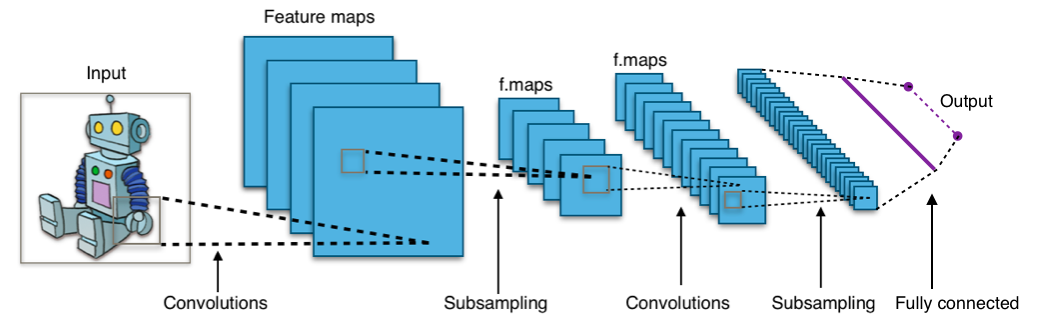
\includegraphics[width=0.9\linewidth]{images/typical_cnn}
    \caption{Typical architecture of a Convolutional Neural Network (CNN). Early layers (left) extract local features such as edges and textures via small convolutional kernels, while deeper layers progressively aggregate these into more global representations of shapes and contextual patterns (right). Adapted from~\cite{wikimedia_typical_cnn}.
    \label{fig:typical_cnn}}
\end{figure}

From a functional perspective, CNNs exploit local connectivity and weight sharing, whereby the same kernel parameters are applied across all spatial locations to efficiently model spatially localized patterns such as edges, textures, and small-scale structures that are ubiquitous in radargrams.
The depth of the network controls the size of the effective receptive field and thus the range of spatial dependencies that can be captured: early layers capture local features and fine-scale patterns (e.g., speckle, small hyperbolas), while deeper layers integrate these into more global representations of shapes and broader contextual patterns (e.g., extended stratigraphic horizons, large-scale clutter distributions).
These properties make CNN-based architectures naturally suited for both deterministic tasks (e.g., denoising, segmentation) and generative modelling of RS data.

\subsection{Encoder–Decoder Architectures (U-Net)}
For tasks like image-to-image translation and semantic segmentation, preserving spatial information is vital. The U-Net architecture~\cite{Ronneberger_2015} introduces a symmetric encoder–decoder structure:
\begin{itemize}
    \item \textbf{Contracting Path (Encoder):} Captures context and reduces spatial resolution through successive convolution and downsampling operations, progressively increasing the number of feature channels.
    \item \textbf{Expanding Path (Decoder):} Restores spatial resolution for precise localization, typically using transposed convolutions or upsampling followed by convolutions, progressively reducing the number of feature channels.
    \item \textbf{Skip Connections:} Direct links between encoder and decoder layers of the same resolution. These are critical for gradient flow and for recovering fine-grained spatial details lost during downsampling, by concatenating high-resolution feature maps from the encoder with the upsampled features in the decoder.
\end{itemize}

\begin{figure}[t]
    \centering
    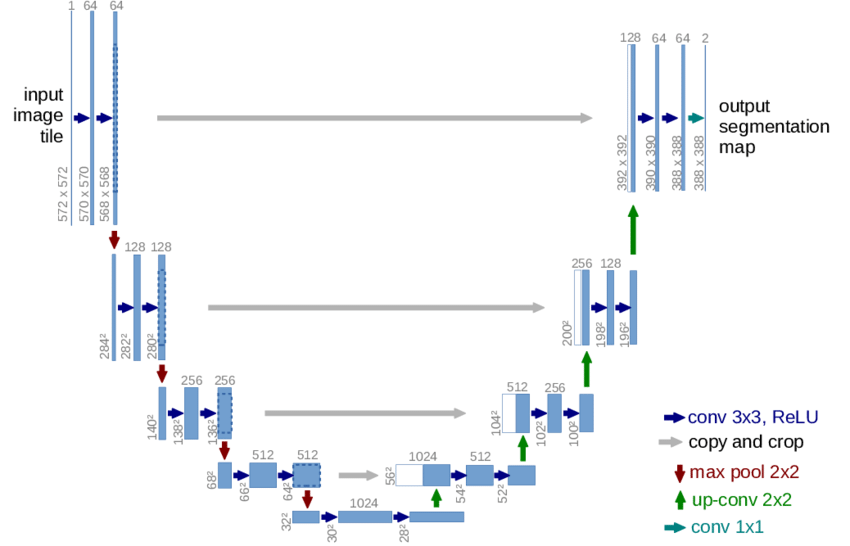
\includegraphics[width=\linewidth]{images/unet_original}
    \caption{Canonical U-Net architecture with a contracting encoder path (left) and a symmetric expanding decoder path (right), connected by skip connections that fuse high-resolution and low-resolution features. Adapted from Figure~1 in~\cite{Ronneberger_2015}.}
    \label{fig:unet_architecture}
\end{figure}

Originally proposed for biomedical image segmentation, U-Net was designed to produce pixel-wise classification maps, effectively performing semantic segmentation by assigning a class label to each pixel.
The combination of a deep encoder (to capture global context) with skip connections (to retain local detail) makes it particularly effective in scenarios where small structures must be delineated precisely against a complex background, while allowing a compact implementation compared to architectures that maintain full spatial resolution throughout the entire network.

In planetary In planetary and terrestrial remote sensing, U-Net-like architectures have been widely adopted for tasks such as crater and impact-structure segmentation, geomorphological mapping, building and road extraction in urban scenes, and land-cover or agricultural field delineation from multispectral imagery, where the goal is to delineate structures (e.g., craters, urban objects, crop parcels, subsurface interfaces) rather than simply classify whole images~\cite{Ronneberger_2015,Ramos2025}.
In the context of this thesis, U-Net plays a dual role:
\begin{itemize}
    \item As  \textbf{generators} in image-to-image translation models such as Pix2Pix, where the encoder–decoder structure is used to map input radargrams (or simulations) to output radargrams while preserving spatial alignment.
    \item As an implicit \textbf{feature extractor for clutter and subsurface structure}, since the multi-scale representation learned by the encoder captures both local patterns (e.g., hyperbolic diffractions, speckle statistics, and pixel textures associated with different subsurface materials) and large-scale stratigraphy, which are essential for the downstream residual-based anomaly detection pipeline.
\end{itemize}

Even when the final output of the generator is an image rather than a segmentation mask, the architectural principles of U-Net ensure that the mapping is spatially consistent: each output pixel is computed from a receptive field that integrates both global context and local detail, an important property when reconstructing physically plausible radargrams from simulated inputs.


\section{Generative Adversarial Networks (GANs)}
\label{sec:gan_theory}
Generative Adversarial Networks (GANs) \cite{Goodfellow_2014} are a class of generative models in which a neural network is trained to synthesize samples that resemble those drawn from a target data distribution.
GANs learn the distribution by framing training as a two-player game between a generator, which produces candidate samples, and a discriminator, which attempts to distinguish real samples from generated ones.
This adversarial formulation has proven particularly effective for high-dimensional image data, where hand-crafted parametric models are often inadequate to capture the full complexity of textures, structures, and noise statistics.
Before discussing conditional extensions and image-to-image translation frameworks, it is useful to formalize this adversarial interaction as a minimax game between generator and discriminator.

\subsection{The Minimax Game}
At the core of a GAN there are two neural networks with opposing objectives:
\begin{itemize}
    \item \textbf{Generator ($G$):} maps a latent vector $z \sim p_z(z)$ (typically a low-dimensional random variable, e.g., Gaussian or uniform) or a structured input (e.g., an image) to a synthetic sample $G(z)$ in the data space. The goal of $G$ is to produce samples that are indistinguishable from real data drawn from the true data distribution $p_{data}$.
    \item \textbf{Discriminator ($D$):} maps an input sample $x$, which may originate from either the real data distribution $p_{data}$ or the generator $G$, to a scalar $D(x) \in (0,1)$, interpreted as the probability that $x$ comes from the true data distribution $p_{data}$ rather than from the generator. The goal of $D$ is to correctly classify real versus generated samples.
\end{itemize}

The training process is formulated as a minimax two-player game with the value function $V(D, G)$ defined as:

\begin{align}
    &\text{Discriminator Objective:} & \max_D V(D, G) &= \mathbb{E}_{x \sim p_{data}(x)}[\log D(x)] + \mathbb{E}_{z \sim p_z(z)}[\log (1 - D(G(z)))] \\
    &\text{Generator Objective:} & \min_G V(D, G) &= \mathbb{E}_{z \sim p_z(z)}[\log (1 - D(G(z)))]
\end{align}

During training, $D$ is updated to maximize $V(D, G)$, i.e., to assign high scores to real samples and low scores to generated samples, while $G$ is updated to minimize $V(D, G)$, i.e., to generate samples that make $D(G(z))$ as large as possible.

In practice, different variants of this objective are often used to improve gradient properties.
A common choice is the \enquote{non-saturating} generator loss, where $G$ maximizes $\mathbb{E}_{z}[\log D(G(z))]$ instead of minimizing $\mathbb{E}_{z}[\log (1 - D(G(z)))]$, leading to stronger gradients when the discriminator is confident.
Other GAN variants (e.g., Wasserstein GANs~\cite{Arjovsky2017}, least-squares GANs~\cite{Mao2017}) modify the loss to stabilize training and improve convergence, and are widely adopted in the broader state of the art for image generation.

From a game-theoretic perspective, the ideal solution of this minimax game is a Nash equilibrium, a pair $(G^*, D^*)$ such that neither player can unilaterally improve its objective given the strategy of the other.
Under suitable assumptions and infinite model capacity, it can be shown that:
\begin{itemize}
    \item The optimal discriminator for a fixed generator is
    \begin{equation}
    D^*(x) = \frac{p_{data}(x)}{p_{data}(x) + p_g(x)},
    \end{equation}
    where $p_g$ is the distribution induced by $G$.
    \item The global optimum of the game is achieved when $p_g = p_{data}$, i.e., the generator distribution matches the true data distribution and $D^*(x) = 0.5$ for all $x$.
\end{itemize}
In this situation, the discriminator cannot distinguish real from generated samples better than random guessing, and the generator produces samples that are statistically indistinguishable from real data.
In practice, GAN training rarely reaches this ideal equilibrium due to limited model capacity, optimization difficulties, and non-convexity, but the framework provides a powerful conceptual tool for designing generative models for complex data such as radargrams.

\subsection{Image-to-Image Translation}
The original GAN formulation is \emph{unconditional}: the generator learns to map random noise $z$ to samples that follow the marginal data distribution $p_{data}(x)$, without explicit control over the content of generated outputs.
In many practical applications, however, we are interested in learning a conditional distribution $p(y \mid x)$: given an input image $x$ (e.g., in our case, a simulated radargram), we wish to generate a corresponding output image $y$ (e.g., a realistic radargram) that preserves the structural content of $x$ while matching the style or statistics of a target domain.
This task is known as \textbf{image-to-image (I2I) translation}.

Examples of I2I tasks include semantic label map $\rightarrow$ RGB image synthesis (and the inverse mapping, i.e., semantic segmentation), grayscale $\rightarrow$ colorization, low-resolution $\rightarrow$ high-resolution super-resolution, or, in this thesis, simulated RS data $\rightarrow$ real RS data.
In all these cases, the model must learn a structured mapping $G: X \to Y$ between two image domains, rather than sampling from $p_{data}(y)$ in isolation.

Conditional GANs (cGANs) extend the basic GAN framework to model such conditional distributions.
Instead of learning $p_g(x)$, a cGAN learns $p_g(y \mid x)$ by conditioning both the generator and the discriminator on the input $x$:
\begin{itemize}
    \item The generator $G$ receives $x$ (and optionally noise $z$) and outputs $G(x, z)$, an image in the target domain.
    \item The discriminator $D$ receives a pair $(x, y)$ and must decide whether $y$ is a real target image paired with $x$, or a generated sample $G(x, z)$.
\end{itemize}
The adversarial objective becomes:
\begin{equation}\label{eq:cgan_objective}
\mathcal{L}_{cGAN}(G, D) = \mathbb{E}_{x,y}[\log D(x, y)] + \mathbb{E}_{x,z}[\log (1 - D(x, G(x, z)))].
\end{equation}

Compared to the unconditional GAN objective, the discriminator now evaluates consistency between input and output, rather than realism of the output alone.
This encourages the generator to produce images that are not only visually plausible in isolation, but also semantically aligned with the conditioning input.
In practice, cGANs are often combined with additional reconstruction losses (e.g., $\ell_1$ or $\ell_2$ between $G(x)$ and $y$) to further enforce fidelity to the input structure, as done in Pix2Pix and in the supervised Sim-to-Real translation experiments of this thesis.

\subsection{Conditional GANs (cGANs)}
\label{subsec:c_gan}


In this formulation, the discriminator receives input–output pairs and learns to distinguish real pairs $(x, y)$ from synthetic pairs $(x, G(x, z))$.
The generator, in turn, is encouraged to produce outputs that are both realistic and appropriately matched to the inputs.

Pix2Pix~\cite{Isola_2017} is a canonical example of a cGAN-based I2I translation model.
It combines the adversarial loss $\mathcal{L}_{cGAN}$ with an $\ell_1$ reconstruction loss
\begin{equation}
\mathcal{L}_{\ell_1}(G) = \mathbb{E}_{x,y}\left[ \| y - G(x) \|_1 \right],
\end{equation}
yielding the overall objective
\begin{equation}
\min_G \max_D \ \mathcal{L}_{cGAN}(G, D) + \lambda \mathcal{L}_{\ell_1}(G),
\end{equation}
where $\lambda$ balances perceptual realism against faithfulness to the ground truth.
In this thesis, Pix2Pix is used as a supervised baseline to translate simulated RS radargrams into the domain of real SHARAD observations, exploiting the availability of paired examples over Elysium Planitia.

\subsection{CycleGAN}
\label{subsec:cyclegan}
For many applications, including planetary RS, paired training data $(x, y)$ are scarce or unavailable: we may have a set of simulated images $X$ and a separate set of real images $Y$, but no one-to-one correspondence between them.
CycleGAN~\cite{Zhu_2017} addresses this setting by learning two mappings $G: X \to Y$ and $F: Y \to X$ together with two discriminators $D_Y$ and $D_X$:
\begin{itemize}
    \item $D_Y$ distinguishes real images $y \in Y$ from translated images $G(x)$.
    \item $D_X$ distinguishes real images $x \in X$ from translated images $F(y)$.
\end{itemize}
Adversarial losses are defined in each domain, encouraging $G$ and $F$ to produce samples that are indistinguishable from real images in $Y$ and $X$, respectively.
To avoid arbitrary mappings that ignore the input content, CycleGAN introduces the \textbf{cycle-consistency loss}:
\begin{equation}
\mathcal{L}_{cyc}(G, F) = \mathbb{E}_{x \sim X}\left[ \| F(G(x)) - x \|_1 \right] + \mathbb{E}_{y \sim Y}\left[ \| G(F(y)) - y \|_1 \right].
\end{equation}
This loss enforces that translating an image from one domain to the other and back again should approximately recover the original, thereby preserving structural information.

The full CycleGAN objective combines adversarial and cycle-consistency terms, and optionally additional regularizers (e.g., identity loss).
In this thesis, CycleGAN is used to perform unpaired Sim-to-Real translation between simulated and real RS radargrams, enabling the generator to learn the statistics of clutter and noise in the real domain without requiring perfectly aligned simulation–observation pairs.

\subsection{Challenges in Training}
\label{subsec:gan_challenges}
GAN training is notoriously unstable due to the non-convex, high-dimensional optimization landscape and the competing objectives of the two networks.
Several failure modes are commonly observed, particularly when training on complex data such as radargrams.
Below we describe the main challenges and established mitigation strategies.

\begin{itemize}
    \item \textbf{Mode Collapse:} The generator collapses to producing only a limited subset of the data distribution (e.g., a single \enquote{average} radargram texture), fooling the discriminator but failing to capture the full diversity of clutter patterns, stratigraphy, and noise statistics in RS data. This is particularly problematic for high-dimensional images where the generator can easily overfit to the most salient samples.

    Possible mitigation techniques are:
    \begin{itemize}
        \item \textbf{Spectral normalization} or \textbf{gradient penalty} on the discriminator to enforce Lipschitz continuity and prevent it from becoming too powerful.
        \item \textbf{Mini-batch discrimination} using statistics (e.g., variance) rather than per-sample classification.
        \item \textbf{Unrolled GANs} or \textbf{progressive growing}, where the discriminator is trained for multiple steps per generator update.
        \item \textbf{Auxiliary losses} such as feature matching, where the generator is encouraged to match intermediate features of the discriminator rather than its final output.
    \end{itemize}

    \item \textbf{Vanishing Gradients:} When the discriminator becomes too confident ($D(G(z)) \approx 0$), the generator receives vanishingly small gradients from the standard loss $\log(1 - D(G(z)))$, halting learning.

    Possible mitigation techniques are:
    \begin{itemize}
        \item \textbf{Non-saturating loss} for the generator: maximize $\log D(G(z))$ instead of minimizing $\log(1 - D(G(z)))$.
        \item \textbf{Label smoothing}, where real samples are assigned soft labels (e.g., $D(x) = 0.9$ instead of $1.0$) to prevent overconfidence.
        \item \textbf{Noise injection} in the discriminator input or \textbf{dropout} to maintain gradient flow.
    \end{itemize}

    \item \textbf{Training Imbalance:} The discriminator can overpower the generator early in training, or vice versa, leading to oscillations or collapse.

    Possible mitigation techniques are:
    \begin{itemize}
        \item \textbf{Adaptive training schedules}: update the weaker network more frequently or use heuristics to pause the stronger one.
        \item \textbf{Wasserstein GANs (WGAN)} \cite{Arjovsky2017}, which replace the Jensen–Shannon divergence with the Wasserstein distance and enforce $1$-Lipschitz continuity via gradient penalty.
        \item \textbf{Two-timescale update rule (TTUR)} \cite{Heusel2017}, where the generator and discriminator have different learning rates and optimizers.
    \end{itemize}

    \item \textbf{Representation Collapse:} The generator learns a representation that is statistically similar to the data but lacks fine semantic details (e.g., blurry radargrams that match average speckle statistics but fail to preserve reflector geometry).

    Possible mitigation techniques are:
    \begin{itemize}
        \item \textbf{Perceptual losses} such as LPIPS or feature matching.
        \item \textbf{Multi-scale discriminators} that operate at different resolutions.
        \item \textbf{Progressive growing of GANs (ProGAN)} \cite{Karras2018}, where the model is trained progressively from low to high resolution.
    \end{itemize}
\end{itemize}

In this thesis, we adopt a combination of Instance Normalization (in the discriminator), Least Squares loss (LSGAN) (for the generator), Label Smoothing, and mixed precision training to stabilize GAN training on RS data.
While more advanced techniques (e.g., WGAN-GP or Spectral Normalization) could be explored in future work, this baseline setup yields robust convergence for both Pix2Pix and CycleGAN on the SHARAD dataset.

A detailed discussion of the evaluation metrics used to assess generative quality in the experimental section of this thesis, including pixel-wise (PSNR, SSIM), perceptual (LPIPS), and domain-specific measures, is provided in Section~\ref{subsec:evaluation_metrics}.


